\section{Infrastruktura komunikacyjna - Message Bus i Message Broker}
\label{sec:infrastrukturaKomunikacyjna}

\par Komunikacja w systemie jest oparta na \emph{RabbitMQ}, który pełni funkcję \emph{Message Broker}a. To rozwiązanie umożliwia scentralizowanie całego procesu komunikacji w systemie. W ramach tego rozwiązania różne typy wiadomości (zapytania, wydarzenia i komendy) są przypisane do swoich dedykowanych giełd\english{Exchange}. Poszczególne serwisy subskrybują te giełdy, co pozwala im na odbieranie odpowiednich komunikatów. Wiadomości są serializowane do formatu \texttt{JSON}. Podczas inicjalizacji systemu, automatycznie tworzone są wszystkie kolejki i giełdy wiadomości.

\par W projekcie wykorzystano wzorzec \emph{Message Bus}, który tworzy warstwę abstrakcji dla komunikacji. Serwisy nie są zobowiązane do świadomości, do którego dokładnie adresata kierują komunikat, aby go dostarczyć, jak i są niezależne od konkretnego \emph{Message Broker}a. Jest to zadaniem konkretnej implementacji \texttt{IMessageBus}, aby skierować wiadomości w odpowiednie miejsce. W projekcie skorzystano z implementacji wzorca pochodzącej z \emph{open source}owej biblioteki \emph{parshim/MessageBus}\cite{PARSHIM_MESSAGEBUS_GITHUB}. Wybór tej konkretnej implementacji wynikał z jej zdolności do kierowania wiadomościami nie tylko na podstawie ich typów, ale także ich treści. Była to istotna cecha, biorąc pod uwagę, że w systemie działa wiele kopii tego samego serwisu (na przykład w przypadku patroli), które są w stanie obsłużyć ten sam typ wiadomości. Serwisy korzystające z \emph{Message Broker}a prezentuje grafika \ref{fig:infrastructureServicesRabbitMq}, natomiast na rysunku \ref{fig:infrastructureRabbitMqExchanges} widzimy utworzone przez system giełdy.

\begin{figure}
    \centering
    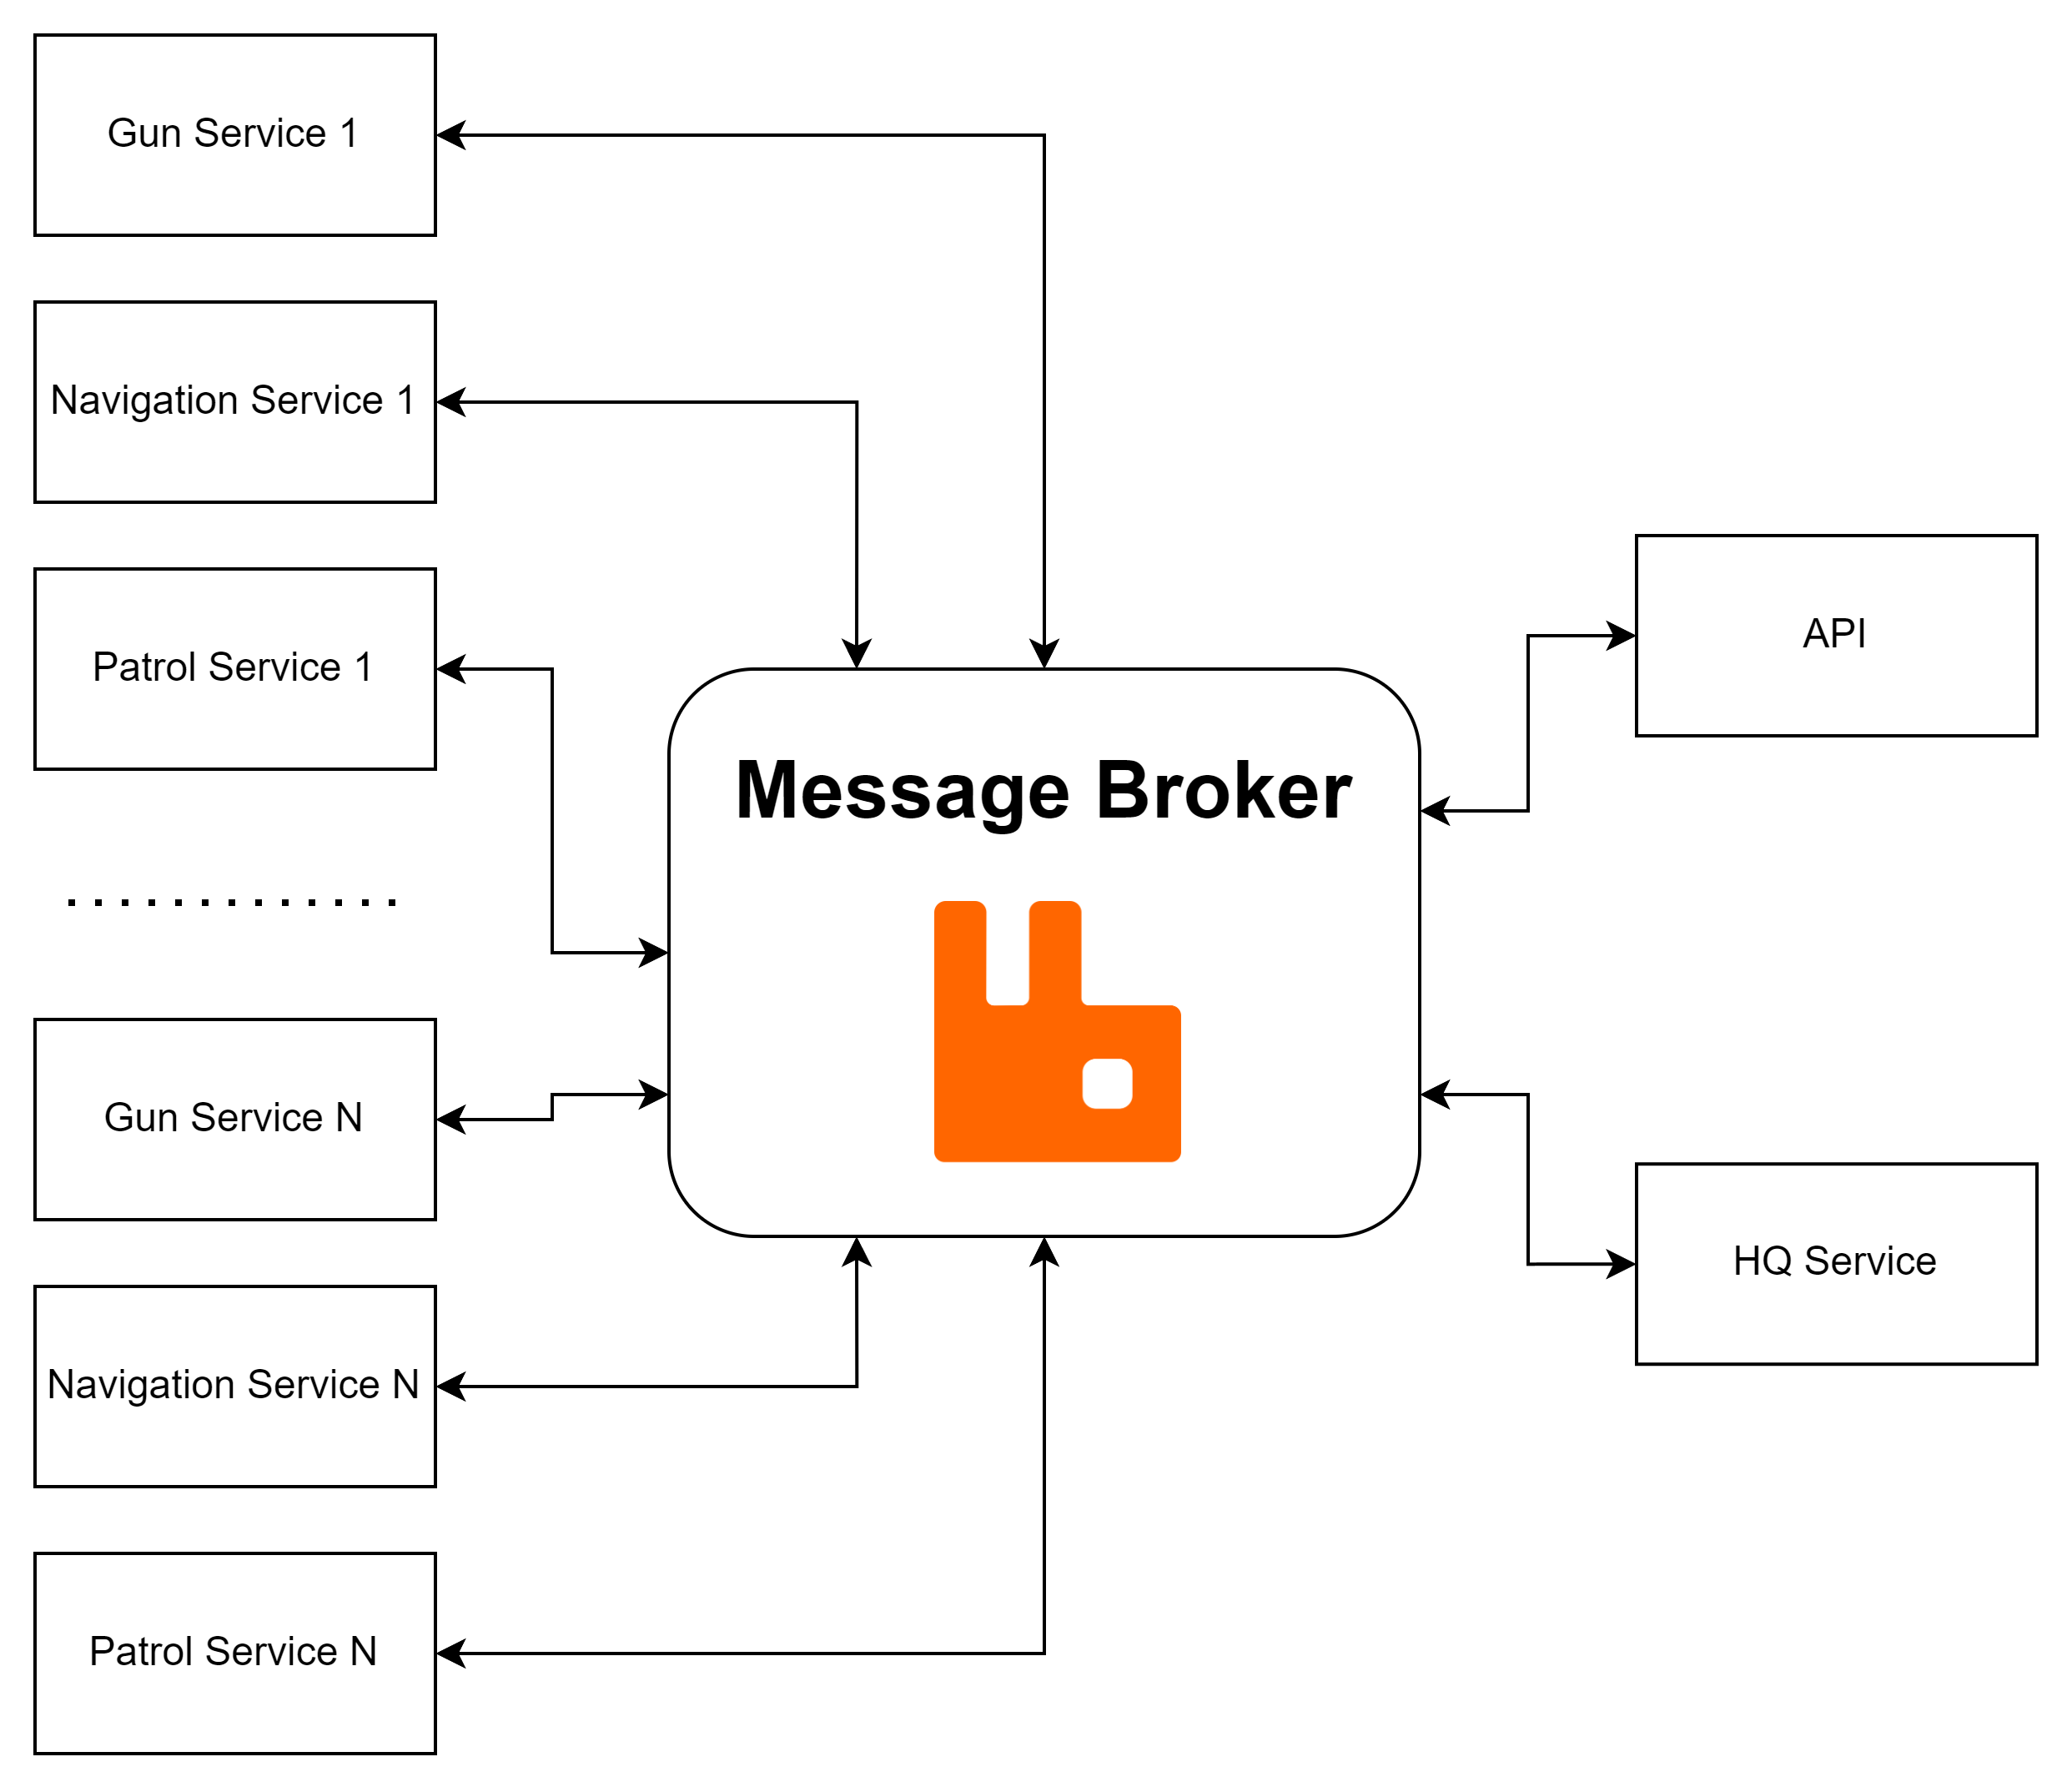
\includegraphics[width=\linewidth]{Infrastructure - Services - RabbitMQ}
    \caption{Diagram przedstawiający serwisy korzystające z \emph{Message Broker}a}
    \label{fig:infrastructureServicesRabbitMq}
    \source{Opracowanie Własne}
\end{figure}

\begin{figure}
    \centering
    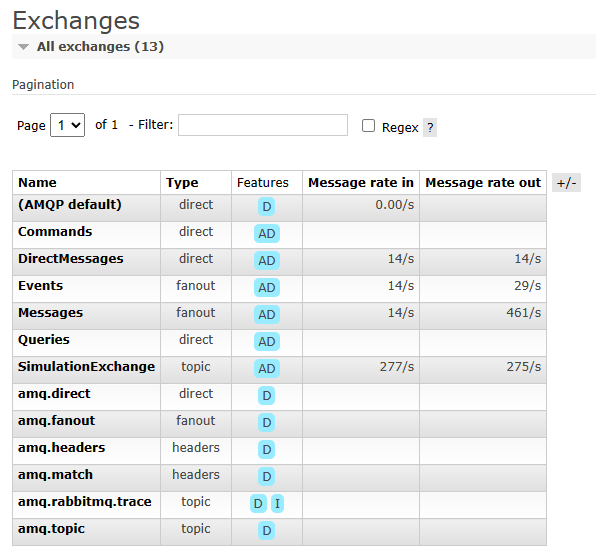
\includegraphics[width=\linewidth]{Infrastructure - RabbitMQ Exchanges}
    \caption{Giełdy w \emph{RabbitMQ} utworzone przez system}
    \label{fig:infrastructureRabbitMqExchanges}
    \source{Opracowanie Własne}
\end{figure}

\par Wiadomości w systemie zostały podzielone na kwerendy\english{Query}, komendy\english{Command} i wydarzenie\english{Event}. Dodatkowo agenci porozumiewają się wiadomościami implementującymi interfejs \texttt{IMessage}, a komunikacja z symulacją odbywa się przy wykorzystaniu komunikatów implementujących \texttt{ISimulationMessage}.

\par Zapytania wysyłane pomiędzy serwisami implementują specjalny interfejs \texttt{IQuery<out TResult>}, który pozwala na wyspecyfikowanie typu oczekiwanego rezultatu. Są wykorzystywane do odpytania innego serwisu w celu uzyskania od niego informacji. System zakłada, że będzie tylko jeden odbiorca takiej wiadomości. Powinien on zostać podany w polu \texttt{Receiver}.

\par Komendy mogą, ale nie muszą zwracać wyniku. Dlatego zostały przygotowane dla nich dwa interfejsy: \texttt{ICommand} i \texttt{ICommand<out TResult>}. Zadaniem tych wiadomości jest wywołanie procesu w innym serwisie, jak i otrzymanie informacji o jego zakończeniu wraz z wynikiem.

\par Zdarzenia w systemie mogą być lokalne lub integracyjne\english{Integration}. To właśnie te drugie, są propagowane w systemie z wykorzystaniem interfejsu \texttt{IEvent}. Ich zadaniem jest poinformowanie o zmianach, jakie zachodzą w systemie. W przypadku zdarzeń, nie oczekuje się na ich rezultat. Są one publikowane w systemie \emph{Fire and Forget}. Odbiorcami są wszystkie serwisy zainteresowane i będące w stanie obsłużyć dane zdarzenie.

\par Wszystkie opisane powyżej typy wiadomości są obsługiwane przez tak zwane \emph{Handler}y, które spełniają jeden z intefejsów: \texttt{IEventHandler<in TEvent>}, \texttt{ICommandHandler<in TCommand, TResult>}, \texttt{ICommandHandler<in TCommand>} lub \texttt{IQueryHandler<in TQuery, TResult>} w zależności od typu danej wiadomości. Klasy spełniające wcześniej wymienione interfejsy są automatycznie znajdywane w danym \texttt{Assembly} i rejestrowane w kontenerze \emph{IoC}\footnote{Inversion of Control}. Rozwiązanie to można porównać do \emph{Event-Driven Architecture}, oczywiście rozszerzonej o komendy i zapytania. Zastosowanie tego rozwiązania pozwoliło w zdecydowanym stopniu zmniejszyć stopień zależności\english{Decoupling} w systemie.

\par Dodatkowo w systemie występują również agenci, ich implementacja została dokładniej omówiona w podrozdziale \ref{sec:implementacjaAgentow}. Komunikacja pomiędzy nimi opiera się na interfejsie \texttt{IMessage}, który został zdefiniowany w taki sposób, aby być otwartym na rozszerzenia i możliwość implementacji własnych mechanizmów opartych o informacje w nim zawarte. Jedną z tych informacji jest pole \texttt{Receivers}, które jest opcjonalne. Jeżeli zawiera ono jaką wartość, to powinna to być lista odbiorców, do których skierowana jest dana wiadomość. W ten sposób \emph{Message Bus} jest w stanie wysłać do nich wiadomość w sposób bezpośredni. Istotnymi są również pola \texttt{MessageId} i \texttt{ResponseTo}, pozwalające na prowadzenie wymiany wiadomości w sposób zorganizowany. Na bazie tych informacji agenci implementują mechanizmy potwierdzania obsłużenia wiadomości i pytania siebie na wzajem o informacje, dokładniej opisane w podrozdziale \ref{sec:implementacjaAgentow}.

\par Symulacja, dokładniej opisana w podrozdziale \ref{sec:symulacja}, również wymaga komunikacji z serwisami działającym w systemie. Odbywa się to przy wykorzystaniu osobnego \emph{Service Bus}a. Możliwym byłoby zastosowanie do tego osobnego \emph{Message Broker}a, jednak tutaj nie zachodziła taka potrzeba, dlatego ta sama instancja \emph{RabbitMQ} obsługuje tę wymianę informacji. Wiadomości spełniające interfejs \texttt{ISimulationMessage} mogą zarówno zostać wysłane przez symulację do danego odbiorcy, jak i zostać do niej nadane, celem poinformowania o podjętej akcji. Dodatkowo został tutaj również wykorzystany mechanizm kwerend, ze względu na konieczność pozyskania informacji o dostępnych dzielnicach\english{District} w mieście przez \emph{HQ Service}.